\documentclass[a4paper,twocolumn]{article}

\usepackage[margin=1in]{geometry}
\usepackage[utf8]{inputenc}
\usepackage[T1]{fontenc}
\usepackage{mathrsfs}
\usepackage{textcomp}
\usepackage[french]{babel}
\usepackage{amsmath}
\usepackage{amssymb}
\usepackage{cancel}
\usepackage{frcursive}
\usepackage[inline]{asymptote}
\usepackage{tikz}
\usepackage[european,straightvoltages,europeanresistors]{circuitikz}
\usepackage{tikz-cd}
\usepackage{tkz-tab}
\usepackage[b]{esvect}
\usepackage[framemethod=TikZ]{mdframed}
\usepackage{centernot}
\usepackage{diagbox}
\usepackage{dsfont}
\usepackage{fancyhdr}
\usepackage{float}
\usepackage{graphicx}
\usepackage{listings}
\usepackage{multicol}
\usepackage{nicematrix}
\usepackage{pdflscape}
\usepackage{stmaryrd}
\usepackage{xfrac}
\usepackage{hep-math-font}
\usepackage{amsthm}
\usepackage{thmtools}
\usepackage{indentfirst}
\usepackage[framemethod=TikZ]{mdframed}
\usepackage{accents}
\usepackage{soulutf8}
\usepackage{mathtools}
\usepackage{bodegraph}
\usepackage{slashbox}
\usepackage{enumitem}
\usepackage{calligra}
\usepackage{cinzel}
\usepackage{BOONDOX-calo}

% Tikz
\usetikzlibrary{babel}
\usetikzlibrary{positioning}
\usetikzlibrary{calc}

% global settings
\frenchspacing
\reversemarginpar
\setuldepth{a}

%\everymath{\displaystyle}

\frenchbsetup{StandardLists=true}

\def\asydir{asy}

%\sisetup{exponent-product=\cdot,output-decimal-marker={,},separate-uncertainty,range-phrase=\;à\;,locale=FR}

\setlength{\parskip}{1em}

\theoremstyle{definition}

% Changing math
\let\emptyset\varnothing
\let\ge\geqslant
\let\le\leqslant
\let\preceq\preccurlyeq
\let\succeq\succcurlyeq
\let\ds\displaystyle
\let\ts\textstyle

\newcommand{\C}{\mathds{C}}
\newcommand{\R}{\mathds{R}}
\newcommand{\Z}{\mathds{Z}}
\newcommand{\N}{\mathds{N}}
\newcommand{\Q}{\mathds{Q}}

\renewcommand{\O}{\emptyset}

\newcommand\ubar[1]{\underaccent{\bar}{#1}}

\renewcommand\Re{\expandafter\mathfrak{Re}}
\renewcommand\Im{\expandafter\mathfrak{Im}}

\let\slantedpartial\partial
\DeclareRobustCommand{\partial}{\text{\rotatebox[origin=t]{20}{\scalebox{0.95}[1]{$\slantedpartial$}}}\hspace{-1pt}}

% merging two maths characters w/ \charfusion
\makeatletter
\def\moverlay{\mathpalette\mov@rlay}
\def\mov@rlay#1#2{\leavevmode\vtop{%
   \baselineskip\z@skip \lineskiplimit-\maxdimen
   \ialign{\hfil$\m@th#1##$\hfil\cr#2\crcr}}}
\newcommand{\charfusion}[3][\mathord]{
    #1{\ifx#1\mathop\vphantom{#2}\fi
        \mathpalette\mov@rlay{#2\cr#3}
      }
    \ifx#1\mathop\expandafter\displaylimits\fi}
\makeatother

% custom math commands
\newcommand{\T}{{\!\!\,\top}}
\newcommand{\avrt}[1]{\rotatebox{-90}{$#1$}}
\newcommand{\bigcupdot}{\charfusion[\mathop]{\bigcup}{\cdot}}
\newcommand{\cupdot}{\charfusion[\mathbin]{\cup}{\cdot}}
%\newcommand{\danger}{{\large\fontencoding{U}\fontfamily{futs}\selectfont\char 66\relax}\;}
\newcommand{\tendsto}[1]{\xrightarrow[#1]{}}
\newcommand{\vrt}[1]{\rotatebox{90}{$#1$}}
\newcommand{\tsup}[1]{\textsuperscript{\underline{#1}}}
\newcommand{\tsub}[1]{\textsubscript{#1}}

\renewcommand{\mod}[1]{~\left[ #1 \right]}
\renewcommand{\t}{{}^t\!}
\newcommand{\s}{\text{\calligra s}}

% custom units / constants
%\DeclareSIUnit{\litre}{\ell}
\let\hbar\hslash

% header / footer
\pagestyle{fancy}
\fancyhead{} \fancyfoot{}
\fancyfoot[C]{\thepage}

% fonts
\let\sc\scshape
\let\bf\bfseries
\let\it\itshape
\let\sl\slshape

% custom math operators
\let\th\relax
\let\det\relax
\DeclareMathOperator*{\codim}{codim}
\DeclareMathOperator*{\dom}{dom}
\DeclareMathOperator*{\gO}{O}
\DeclareMathOperator*{\po}{\text{\cursive o}}
\DeclareMathOperator*{\sgn}{sgn}
\DeclareMathOperator*{\simi}{\sim}
\DeclareMathOperator{\Arccos}{Arccos}
\DeclareMathOperator{\Arcsin}{Arcsin}
\DeclareMathOperator{\Arctan}{Arctan}
\DeclareMathOperator{\Argsh}{Argsh}
\DeclareMathOperator{\Arg}{Arg}
\DeclareMathOperator{\Aut}{Aut}
\DeclareMathOperator{\Card}{Card}
\DeclareMathOperator{\Cl}{\mathcal{C}\!\ell}
\DeclareMathOperator{\Cov}{Cov}
\DeclareMathOperator{\Ker}{Ker}
\DeclareMathOperator{\Mat}{Mat}
\DeclareMathOperator{\PGCD}{PGCD}
\DeclareMathOperator{\PPCM}{PPCM}
\DeclareMathOperator{\Supp}{Supp}
\DeclareMathOperator{\Vect}{Vect}
\DeclareMathOperator{\argmax}{argmax}
\DeclareMathOperator{\argmin}{argmin}
\DeclareMathOperator{\ch}{ch}
\DeclareMathOperator{\com}{com}
\DeclareMathOperator{\cotan}{cotan}
\DeclareMathOperator{\det}{det}
\DeclareMathOperator{\id}{id}
\DeclareMathOperator{\rg}{rg}
\DeclareMathOperator{\rk}{rk}
\DeclareMathOperator{\sh}{sh}
\DeclareMathOperator{\th}{th}
\DeclareMathOperator{\tr}{tr}

% colors and page style
\definecolor{truewhite}{HTML}{ffffff}
\definecolor{white}{HTML}{faf4ed}
\definecolor{trueblack}{HTML}{000000}
\definecolor{black}{HTML}{575279}
\definecolor{mauve}{HTML}{907aa9}
\definecolor{blue}{HTML}{286983}
\definecolor{red}{HTML}{d7827e}
\definecolor{yellow}{HTML}{ea9d34}
\definecolor{gray}{HTML}{9893a5}
\definecolor{grey}{HTML}{9893a5}
\definecolor{green}{HTML}{a0d971}

\pagecolor{white}
\color{black}

\begin{asydef}
	settings.prc = false;
	settings.render=0;

	white = rgb("faf4ed");
	black = rgb("575279");
	blue = rgb("286983");
	red = rgb("d7827e");
	yellow = rgb("f6c177");
	orange = rgb("ea9d34");
	gray = rgb("9893a5");
	grey = rgb("9893a5");
	deepcyan = rgb("56949f");
	pink = rgb("b4637a");
	magenta = rgb("eb6f92");
	green = rgb("a0d971");
	purple = rgb("907aa9");

	defaultpen(black + fontsize(8pt));

	import three;
	currentlight = nolight;
\end{asydef}

% theorems, proofs, ...

\mdfsetup{skipabove=1em,skipbelow=1em, innertopmargin=6pt, innerbottommargin=6pt,}

\declaretheoremstyle[
	headfont=\normalfont\itshape,
	numbered=no,
	postheadspace=\newline,
	headpunct={:},
	qed=\qedsymbol]{demstyle}

\declaretheorem[style=demstyle, name=Démonstration]{dem}

\newcommand\veczero{\kern-1.2pt\vec{\kern1.2pt 0}} % \vec{0} looks weird since the `0' isn't italicized

\makeatletter
\renewcommand{\title}[2]{
	\AtBeginDocument{
		\begin{titlepage}
			\begin{center}
				\vspace{10cm}
				{\Large \sc Chapitre #1}\\
				\vspace{1cm}
				{\Huge \calligra #2}\\
				\vfill
				Hugo {\sc Salou} MPI${}^{\star}$\\
				{\small Dernière mise à jour le \@date }
			\end{center}
		\end{titlepage}
	}
}

\newcommand{\titletp}[4]{
	\AtBeginDocument{
		\begin{titlepage}
			\begin{center}
				\vspace{10cm}
				{\Large \sc tp #1}\\
				\vspace{1cm}
				{\Huge \textsc{\textit{#2}}}\\
				\vfill
				{#3}\textit{MPI}${}^{\star}$\\
			\end{center}
		\end{titlepage}
	}
	\fancyfoot{}\fancyhead{}
	\fancyfoot[R]{#4 \textit{MPI}${}^{\star}$}
	\fancyhead[C]{{\sc tp #1} : #2}
	\fancyhead[R]{\thepage}
}

\newcommand{\titletd}[2]{
	\AtBeginDocument{
		\begin{titlepage}
			\begin{center}
				\vspace{10cm}
				{\Large \sc td #1}\\
				\vspace{1cm}
				{\Huge \calligra #2}\\
				\vfill
				Hugo {\sc Salou} MPI${}^{\star}$\\
				{\small Dernière mise à jour le \@date }
			\end{center}
		\end{titlepage}
	}
}
\makeatother

\newcommand{\sign}{
	\null
	\vfill
	\begin{center}
		{
			\fontfamily{ccr}\selectfont
			\textit{\textbf{\.{\"i}}}
		}
	\end{center}
	\vfill
	\null
}

\renewcommand{\thefootnote}{\emph{\alph{footnote}}}

% figure support
\usepackage{import}
\usepackage{xifthen}
\pdfminorversion=7
\usepackage{pdfpages}
\usepackage{transparent}
\newcommand{\incfig}[1]{%
	\def\svgwidth{\columnwidth}
	\import{./figures/}{#1.pdf_tex}
}

\pdfsuppresswarningpagegroup=1
\ctikzset{tripoles/european not symbol=circle}

\newcommand{\missingpart}{{\large\color{red} Il manque quelque chose ici\ldots}}


%\pagecolor{truewhite}
%\color{trueblack}

\titletp{ts 4}{Filtrage analogique d'un signal périodique}
{
	\begin{tabular}{c}
		Hugo {\sc Salou}\/\\
		Alan {\sc Le Brech}\/\\
		Nicolas {\sc Vincent}\/
	\end{tabular}
}{Hugo {\sc Salou}, Alan {\sc Le Brech}\/ et Nicolas {\sc Vincent}}

\begin{document}
	L'objectif de ce {\sc tp}\/ est de réaliser un analyseur de spectre analogique, à base d'un {\sc ali}.
	On réalise un filtre passe-bande qui, en modifiant sa fréquence propre, peut détecter les différentes composantes de la décompositions en séries de {\sc Fourier}\/ du signal.

	\begin{figure}[H]
		\centering\footnotesize
		\begin{circuitikz}[scale=0.8]
			\draw (6,1)node[en amp, noinv input up](E){};
			\draw (0,2) to[R=$R_1$] (2,2) to[C=$C$] (2,4);
			\draw let \p1 = (E.out) in (2,4) -- (\x1,4) -- (E.out);
			\draw (2,2) to[C=$C$] (4,2) to[R=$R_3$] (4,4);
			\draw let \p2 = (E.+) in (2,2) -- (\x2,2) -- (E.+);
			\draw let \p3 = (E.-) in (0,-1) -- (\x3,-1) -- (E.-);
			\draw let \p1 = (E.out) in let \p3 = (E.-) in (\x3,-1) -- (\x1, -1);
			\draw (2,-1) to[R=$R_2$] (2,2);
			\draw[->] (0.1, -0.8) -- (0.1, 1.8);
			\draw (0.3, 0.5) node {$v_\text{e}$};
			\draw (7.5, 0) node {$v_\text{s}$};
			\draw[->] (7.3, -0.8) -- (7.3, 0.8);
		\end{circuitikz}
		\caption{Circuit réalisé durant ce {\sc tp}}
		\label{fig:circuit}
	\end{figure}

	On réalise le circuit décrit dans la figure~\ref{fig:circuit}.
	D'après l'énoncé, la fonction de transfert $\ubar{H}(\mathrm{j}\omega)$\/ de ce circuit est : \[
		\ubar{H}(\mathrm{j}\omega) \triangleq \frac{v_\text{s}}{v_\text{e}} = \frac{H_0}{1 + \mathrm{j}Q\left( \frac{\omega}{\omega_0} - \frac{\omega_0}{\omega} \right)}.
	\] Ainsi, la pulsation $\omega_0$\/ du circuit est donnée par l'expression suivante \[
		\omega_0 = \frac{1}{C} \sqrt{\frac{R_1 + R_2}{R_1R_2R_3}},
	\] et le facteur de qualité $Q$\/ est donné par  \[
		Q = \frac{1}{2}\sqrt{R_3\:\frac{R_1+R_2}{R_1\,R_2}} 
	.\]
	\begin{figure}[H]
		\centering
		\begin{asy}
			import graph;
			size(7.5cm);
			draw((-0.4,0)--(10,0), Arrow(TeXHead));
			draw((0,-0.2) -- (0, 4), Arrow(TeXHead));
			void f(real x, real y) {
				draw((x,0)--(x,y), magenta);
				dot((x,y), magenta);
				label("$" + string(x*200) + "\:\mathrm{Hz}$", (x,0), align=S);
			}
			real g(real x) {
				real u = x - 3;
				return 3.5 * exp(-u*u*10);
			}
			f(1, 3);
			f(3, 2.5);
			f(5, 1.25);
			f(7, 1);
			f(9, 0.75);
			draw(graph(g, 0, 10, 500), deepcyan);
			draw((2.75, g(2.75)) -- (3.25, g(3.25)), Arrows(TeXHead));
			label("$\mathrm{\Delta}\omega$", (2.75, g(2.75)), align=NW);
			label("Amplitude", (0, 4), align=NE);
			label("$\omega$", (10, 0), align=NE);
		\end{asy}
		\caption{Spectre du signal carré et gain du circuit (non à l'échelle)}
		\label{fig:filtre-diag}
	\end{figure}
	On en déduit l'expression de la largeur de la bande passante $\mathrm{\Delta}\omega$\/ (comme montré dans la figure~\ref{fig:filtre-diag}) : \[
		\mathrm{\Delta}\omega = \frac{\omega_0}{Q} = \frac{2}{C\,R_3}
	.\] Comme les valeurs de $R_3$\/ et $C$\/ sont constantes (on ne fait varier que $R_2$), la largeur de la bande passante reste constante.

	On vérifie qu'avec les valeurs des composants, le {\sl cahier des charges}\/ du filtre, donné dans l'énoncé, est respecté.
	On a $R_1 = 470\:\mathrm{k\Omega}$, $R_2 \in [10\:\mathrm{\Omega},10\:\mathrm{k\Omega}]$, $R_3 = 1{,}0\:\mathrm{M\Omega}$, $C = 10\:\mathrm{nF}$. On en déduit les valeurs de $\omega_0$\/ minimales et maximales prisent pour différentes valeurs de $R_2$. On a donc \[
		\omega_{0,\text{max}} \cong 2{,}2\times 10^4\:\mathrm{rad}/\mathrm{s}
	\] et \[
		\omega_{0,\text{min}} \cong 7{,}2\times 10^2\:\mathrm{rad}/\mathrm{s}
	\] d'où \[
		f_{0,\text{max}} = 3{,}6\:\mathrm{kHz}\quad\text{et}\quad f_{0,\text{min}} = 1{,}1\times 10^2\:\mathrm{Hz}
	.\]
	Également, on en déduit la valeur de $\mathrm{\Delta}\omega$\/ du circuit : \[
		\mathrm{\Delta}\omega \cong 2{,}0\times 10^{2}\:\mathrm{rad}/\mathrm{s},\quad\text{d'où},\quad \mathrm{\Delta}f \cong 32\:\mathrm{Hz}
	.\]
	Avec ces spécifications, le circuit respecte donc le~{\sl cahier} {\sl des charges}\/ : on peut isoler des fréquences allant de $100\:\mathrm{Hz}$\/ à $2\:\mathrm{kHz}$\/ avec une précision d'au moins $100\:\mathrm{Hz}$.

	On réalise le circuit de la figure~\ref{fig:circuit} et on règle le signal d'entrée sur un signal créneau de fréquence $200\:\mathrm{Hz}$\/ et d'amplitude $2\:\mathrm{V}$.
	Pour identifier les différentes composantes harmoniques du signal créneau, on mesure à l'oscilloscope le signal $v_\text{s}$, et, en balayant les différentes valeurs de $R_2$, on repère quand le signal observé est sinusoïdal.

	Également, on note les amplitudes des signaux observés, afin d'en déduire les amplitudes $C_n$\/ des harmoniques du signal.

	Les résultats de cette identifications sont montrés dans la table~\ref{tab:res}. On représente également quelques acquisitions dans les figures~\ref{fig:aq1}, \ref{fig:aq2} et~\ref{fig:aq3} (à la fin du document).

	Dans la table~\ref{tab:res}, le terme $A_n$\/ est l'amplitude mesurée $v_\text{s}$\/ pendant l'identification de la $n$ième harmonique.
	Mais, d'après l'énoncé, le gain en $\omega_0$\/ est \[
		|H_0| = \frac{R_3}{2R_1} \mathrel{\mathop=^{(\text{\sc AN})}} 1{,}06
	\] or, comme la valeur de $\omega_0$\/ correspond approximativement à celle de $\omega_n$, la pulsation de la $n$ième harmonique, on en déduit que \[
		\forall n,\qquad A_n = H_0\times C_n
	.\] 

	\begin{table}[H]
		\centering
		\begin{tabular}{|c|c|c|c|}
			\hline
			$n$&$f_n$&$A_n$&$n\times A_n$\\ \hline
			1&$200\:\mathrm{Hz}$&$2{,}7\:\mathrm{V}$&$2{,}7\:\mathrm{V}$\\
			3&$600\:\mathrm{Hz}$&$0{,}85\:\mathrm{V}$&$2{,}5\:\mathrm{V}$\\
			5&$1\,000\:\mathrm{Hz}$&$0{,}35\:\mathrm{V}$&$1{,}8\:\mathrm{V}$\\
			\hline
		\end{tabular}
		\caption{Résultats de l'identification}
		\label{tab:res}
	\end{table}

	On remarque que, pour chaque harmonique~$n$, $n \times A_n = n \times A_n \times H_0$\/ est constant. Or, $H_0$\/ est constant. On en déduit que les amplitudes $C_n$\/ des harmoniques du signal suivent une décroissance en~$\frac{1}{n}$. Mais, dès la cinquième harmonique (donc dès~$1\,000\:\mathrm{Hz}$), nous arrivons aux limites du filtre.

	On détermine également les amplitudes~$C_n$\/ à l'aide de la fonction {\sc fft}\/ de l'oscilloscope et des curseurs, comme représenté sur la figure~\ref{fig:fft}.
	On compare ces nouvelles valeurs avec celles trouvées précédemment.
	On montre ces valeurs dans la table~\ref{tab:res2}.

	\begin{table}[H]
		\centering
		\begin{tabular}{|c|c|c|}
			\hline
			$n$&\sc fft&\sc filtre\\\hline
			1&$2{,}5\:\mathrm{V}$&$2{,}5\:\mathrm{V}$\\
			3&$0{,}81\:\mathrm{V}$&$0{,}80\:\mathrm{V}$\\
			5&$0{,}49\:\mathrm{V}$&$0{,}35\:\mathrm{V}$\\
			7&$0{,}33\:\mathrm{V}$&---\\
			9&$0{,}25\:\mathrm{V}$&---\\ \hline
		\end{tabular}
		\caption{Comparaison des résultats pour les valeurs de $C_n$\/ du circuit avec ceux de la fonction {\sc fft}\/ de l'oscilloscope}
		\label{tab:res2}
	\end{table}

	On remarque que, pour la {\sc fft}, il y a plus de valeurs. En effet, l'oscilloscope peut analyser des fréquences plus élevées que le circuit, et donc plus d'harmoniques. On peut aisément re-vérifier la décroissance en $\frac{1}{n}$\/ des amplitudes $C_n$\/ avec ces nouvelles valeurs plus précises, qui apparaît plus clairement qu'avec les valeurs du filtre. Ce résultat est montré dans la table~\ref{tab:res3}.

	\begin{table}[H]
		\centering
		\begin{tabular}{|c|c|c|c|}
			\hline
			$n$&$f_n$&$A_n$&$n\times A_n$\\ \hline
			1&$200\:\mathrm{Hz}$&$1{,}67\:\mathrm{V}$&$1{,}67\:\mathrm{V}$\\
			3&$600\:\mathrm{Hz}$&$543\:\mathrm{mV}$&$1{,}63\:\mathrm{V}$\\
			5&$1\,000\:\mathrm{Hz}$&$327\:\mathrm{mV}$&$1{,}64\:\mathrm{V}$\\
			7&$1\,400\:\mathrm{Hz}$&$226\:\mathrm{mV}$&$1{,}58\:\mathrm{V}$\\
			9&$1\,600\:\mathrm{Hz}$&$165\:\mathrm{mV}$&$1{,}49\:\mathrm{V}$\\
			\hline
		\end{tabular}
		\caption{Décroissance en $\frac{1}{n}$\/ à l'aide des mesures de la {\sc fft}\/ de l'oscilloscope}
		\label{tab:res3}
	\end{table}

	\begin{figure}[H]
		\centering
		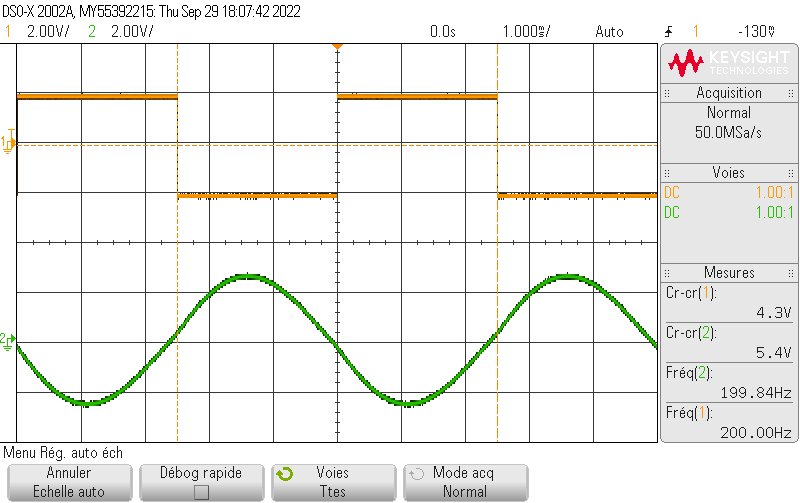
\includegraphics[width=0.45\textwidth]{figures/aq1.png}
		\caption{Acquisition du signal avec un $R_2 = 6{,}4\:\mathrm{k\Omega}$}
		\label{fig:aq1}
	\end{figure}

	\begin{figure}[H]
		\centering
		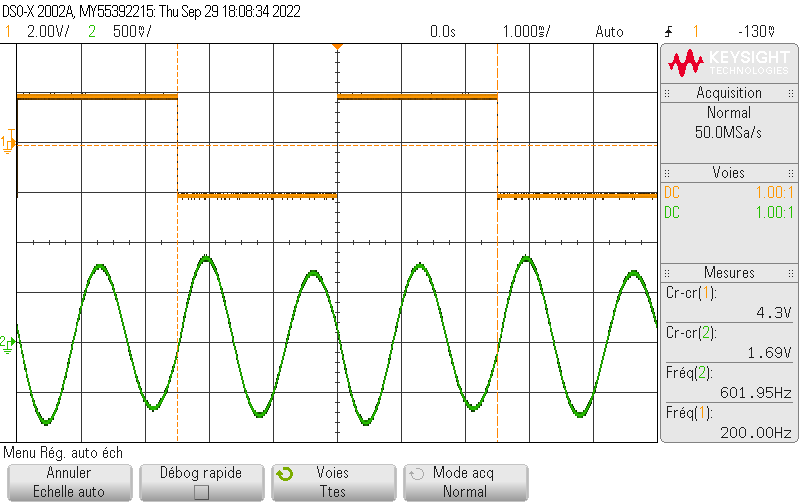
\includegraphics[width=0.45\textwidth]{figures/aq2.png}
		\caption{Acquisition du signal avec un $R_2 = 3{,}8\:\mathrm{k\Omega}$}
		\label{fig:aq2}
	\end{figure}

	\begin{figure}[H]
		\centering
		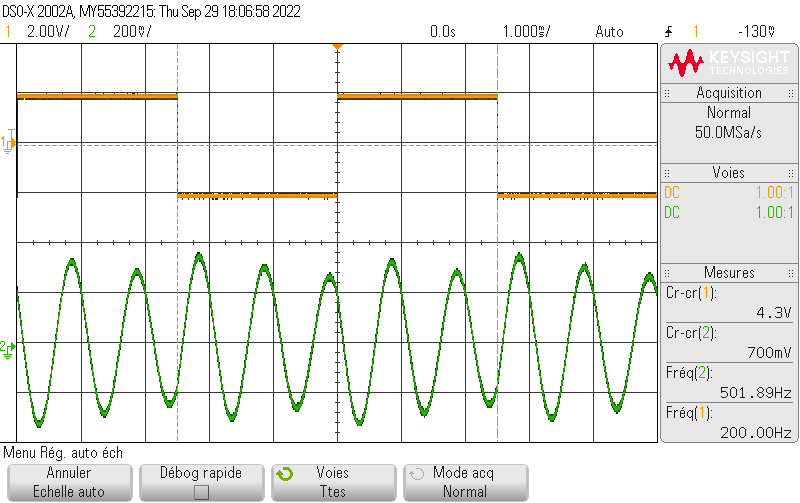
\includegraphics[width=0.45\textwidth]{figures/aq5.png}
		\caption{Acquisition du signal avec un $R_2 = 250\:\mathrm{\Omega}$}
		\label{fig:aq3}
	\end{figure}

	\begin{figure}[H]
		\centering
		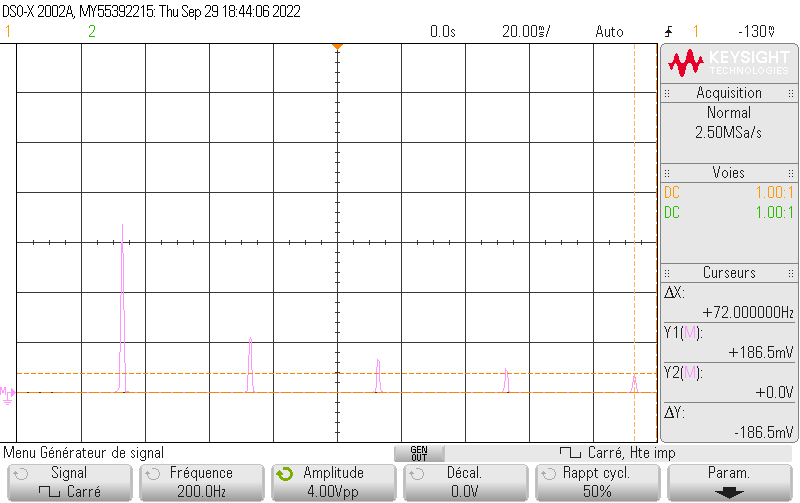
\includegraphics[width=0.45\textwidth]{figures/fft2.png}
		\caption{{\sc fft}\/ du signal $v_\text{s}$}
		\label{fig:fft}
	\end{figure}

	\sign
\end{document}
